% !TEX root=../main.tex
\documentclass[beamer]{standalone}
\begin{document}

% title image
\begin{frame}{Problem statement and Concept}
    \begin{figure}
        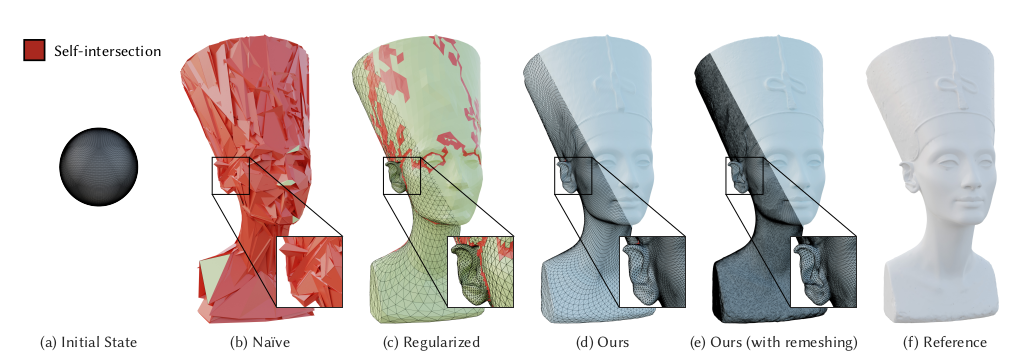
\includegraphics[width=1.0\textwidth]{./figures/intro-figure-1.png}
    \end{figure}

% note %
\note[item] {
    This paper is about mesh optimizing technique using differentiable rendering.

    This is the title image of the paper.
}

\end{frame}

% introduction
\begin{frame}{Problem statement and Concept}
    \begin{itemize}
        \setlength\itemsep{1em}
        \item Problem 
        \begin{enumerate}
            \item \alert{Very fragile} mesh optimizing process - (i.e. learning rate)
            \item Usually stucked to local minimum in the case of mesh optimization in DR
        \end{enumerate}

        \begin{figure}
            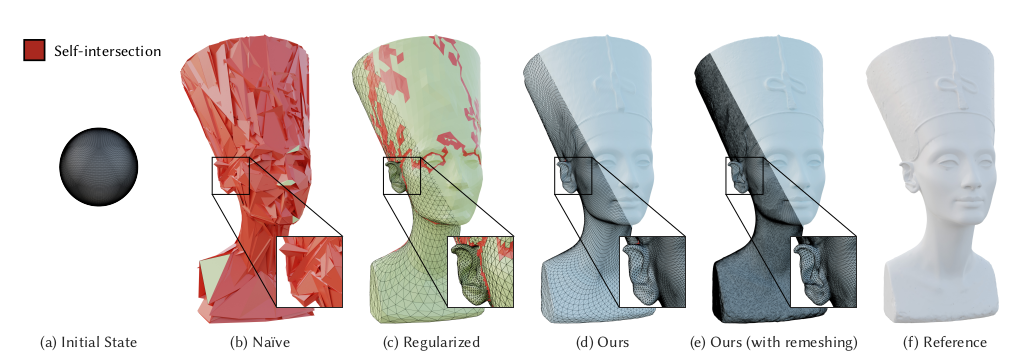
\includegraphics[width=0.65\textwidth]{./figures/intro-figure-1.png}
        \end{figure}

        \pause

        \item Concepts
        \begin{enumerate}
            \item Finding a global optimum (high quailty mesh)
            \item Guarenteed fast convergence speed by taking large steps
            \item The modified laplace gradient filtering in second order optimization method
        \end{enumerate}
    \end{itemize}
    
% notes %
\note[item]{
    In differentiable rendering, It is hard to target optimizing vertex positions. 
    
    This process is very fragile.
    When we attempt to do that, the results of shapes are usually stucked to local minimum.

    As this title image, the naive adpatation make the awful result.
    the initial state is sphere. And the target is Nefertiti. Red represents the face intersections.
}

\note[item] {
    The main goal of this paper is improving this mesh optimizing process.
    
    I choosed the three important concepts of this paper.

    First, Finding a global optimum (high quailty mesh), skipping to be stucked in local minimum
    
    Second, Guarenteed fast convergence speed by large step length
    
    Third, The modified laplace gradient filtering in second order optimization method

    If you remember these things during the presentation, understanding would be easier.
}
\end{frame}
\end{document}